
\begin{figure}[h!]
    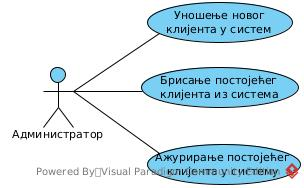
\includegraphics{Slike/SUadministrativniPoslovi.jpg}
    \centering
    \caption{Sluchaj upotrebe: Administrativni poslovi}
    \label{administrativni poslovi}
\end{figure}  
Administrativni poslovi su sluchaj upotrebe u kom administrator formira bazu podataka o klijentima. Uchesnik je administrator sistema. Pretpostavlja se da administrator poseduje sve potrebne podatke o klijentu.
\subsubsection{Sluchaj upotrebe: Unoshenje novog klijenta u sistem}
\begin{itemize}
\item{\textbf{Kratak opis:} Administrator unosi informacije o klijentu koji u trenutku unosa ne postoji u sistemu. Sistem obradjuje informacije, az1urira se stanje sistema i vrac1a povratna informacija o uspeshnosti unosa.}
\item{\textbf{Akteri:} Administrator sistema}
\item{\textbf{Ulaz:} Podaci o klijentu }
\item{\textbf{Izlaz:} Poruka o uspeshnosti unoshenja klijenta u sistem }
\item{\textbf{Preduslovi:} Administrator ima pristup sistemu i poseduje potrebne informacije o novom klijentu. Postoji komunikacija izmedju administratora i klijenta. }
\item{\textbf{Postuslovi:} Uspeshno dodat klijent u sistem.}
\item{\textbf{Glavni tok:} 
\begin{enumerate}
    \item [1.] Administrator pristupa formularu za unos novog klijenta u okviru sistema.
    \item[2.] Administrator popunjava traz1ene podatke o klijentu (naziv kompanije, PIB kompanije, MB kompanije, adresa sedishta i poshtanski broj, broj aktivnih magacina, adrese i poshtanski brojevi aktivnih magacina ).
    \item[3.] Administrator potvrdjuje unos podataka klikom na dugme.
    \item[4.] Sistem validira unete podatke.
    \item[5.] Sistem chuva podatke o novom klijentu.
    \item[6.] Prikazuje se poruka o uspeshnosti akcije.
\end{enumerate}

}
\item{\textbf{Alternativni tokovi:} 
\begin{enumerate}
    \item [A1.] \textbf{Neuspeshna validacija unetih podataka.} Ukoliko u 4. koraku glavnog toka sistem naidje na neispravno popunjeno polje formulara, sistem c1e markirati isto i obavestiti administratora. Administrator ispravlja unos. Proces se nastavlja u 3. koraku glavnog toka.
    \item[A2.] \textbf{Odustajanje.} Administrator u 3. koraku klikom na dugme odbacuje unete podatke i odustaje od unoshenja novog klijenta u sistem. Informacije o klijentu nisu zapamc1ene u sistemu. Proces se zavrshava.
\end{enumerate}
}
\end{itemize}

\subsubsection{Sluchaj upotrebe: Brisanje postojec1eg klijenta iz sistema}

\begin{itemize}
\item{\textbf{Kratak opis:} Administrator brishe postojec1eg klijenta iz sistema. Az1urira se stanje sistema i vrac1a povratna informacija o uspeshnosti akcije.}
\item{\textbf{Akteri:} Administrator sistema}
\item{\textbf{Ulaz:} / }
\item{\textbf{Izlaz:} Poruka o uspeshnosti brisanja klijenta iz sistema }
\item{\textbf{Preduslovi:} Administrator ima pristup sistemu i poseduje potrebne informacije o klijentu. Postoje informacije o klijentu u sistemu.}
\item{\textbf{Postuslovi:} Uspeshno obrisan klijent iz sistema.}
\item{\textbf{Glavni tok:} 
\begin{enumerate}
    \item [1.] Administrator pristupa formularu za brisanje klijenata iz sistema.
    \item[2.] Administrator pretraz1uje bazu klijenata unoshenjem naziva, PIB-a ili MB-a kompanije u polje za pretragu.
    \item[3.] Administrator potvrdjuje unos klikom na dugme za pretragu.
    \item[4.] Sistem validira podatke.
    \item[5.] Sistem pronalazi klijente na osnovu unetih podataka i prikazuje ih.
    \item[6.] Administrator bira jednog od ponudjenih klijenata klikom na istog.
    \item[7.] Klikom na dugme administrator shalje zahtev za brisanje sistemu.
    \item[8.] Sistem brishe informacije o klijentu i az1urira bazu klijenata.
    \item[9.] Prikazuje se poruka o uspeshnosti izvrshene akcije.
\end{enumerate}

}
\item{\textbf{Alternativni tokovi:} 
\begin{enumerate}
    \item [A1.] \textbf{Neuspeshna validacija podataka za pretragu.} Ukoliko u 4. koraku sistem naidje na neispravno popunjeno polje, obaveshtava administratora adekvatnom porukom. Administrator ispravlja unos i proces se nastavlja u 3. koraku glavnog toka.
    \item[A2.] \textbf{Odustajanje.} Administrator u 7. koraku glavnog toka klikom na dugme odustaje od brisanja klijenta. Informacije o klijentu se chuvaju neizmenjene u sistemu. Proces se zavrshava.
\end{enumerate}
}
\end{itemize}

\subsubsection{Sluchaj upotrebe: Az1uriranje postojec1eg klijenta u sistemu}

\begin{itemize}
\item{\textbf{Kratak opis:} Administrator menja podatke o postojec1em klijentu sistema. Az1urira se stanje sistema i vrac1a povratna informacija o uspeshnosti akcije.}
\item{\textbf{Akteri:} Administrator sistema}
\item{\textbf{Ulaz:} Novi podaci o klijent }
\item{\textbf{Izlaz:} Poruka o uspeshnosti izmene podataka o  klijentu sistema }
\item{\textbf{Preduslovi:} Administrator ima pristup sistemu i poseduje potrebne informacije o klijentu. Postoje informacije o klijentu u sistemu.}
\item{\textbf{Postuslovi:} Uspeshno az1uriran klijent.}
\item{\textbf{Glavni tok:} 
\begin{enumerate}
    \item [1.] Administrator pristupa formularu za az1uriranje klijenata.
    \item[2.] Administrator pretraz1uje bazu klijenata unoshenjem naziva, PIB-a ili MB-a kompanije u polje za pretragu.
    \item[3.] Administrator potvrdjuje unos klikom na dugme za pretragu.
    \item[4.] Sistem validira podatke.
    \item[5.] Sistem pronalazi klijente na osnovu unetih podataka i prikazuje ih.
    \item[6.] Administrator bira jednog od ponudjenih klijenata klikom na istog.
    \item[7.] Klikom na dugme za az1uriranje prikazuje se formular sa podacima o klijentu koji se trenutno chuvaju u sistemu.
    \item[8.] Administrator unosi nove podatke o klijentu.
    \item[9.] Klikom na dugme administrator potvrdjuje unos.
    \item[10.] Sistem validira podatke.
    \item[11.] Sistem chuva nove podatke o klijentu u bazi.
    \item[12.] Sistem prikazuje poruku o uspeshnosti izmena.
\end{enumerate}

}
\item{\textbf{Alternativni tokovi:} 
\begin{enumerate}
    \item [A1.] \textbf{Neuspeshna validacija podataka za pretragu.} Ukoliko u 4. koraku sistem naidje na neispravno popunjeno polje, obaveshtava administratora adekvatnom porukom. Administrator ispravlja unos i proces se nastavlja u 3. koraku glavnog toka.
    \item [A2.] \textbf{Neuspeshna validacija novih podataka o klijentu} Ukoliko u 10. koraku sistem naidje na neispravno popunjeno polje, markira ga i obaveshtava administratora adekvatnom porukom. Administrator ispravlja unos i proces se nastavlja u 9.. koraku glavnog toka.
    \item[A2.] \textbf{Odustajanje.} Administrator u 9. koraku glavnog toka klikom na dugme odustaje od unetih izmena. Chuvaju se se neizmenjeni podaci o klijentu u sistemu. Proces se zavrshava.
\end{enumerate}
}
\end{itemize}

Obradjeni sluchajevi upotrebe iz tekuc1e sekcije se mogu predstaviti narednim BPMN dijagramom.
\newpage

\begin{figure}[h!]
    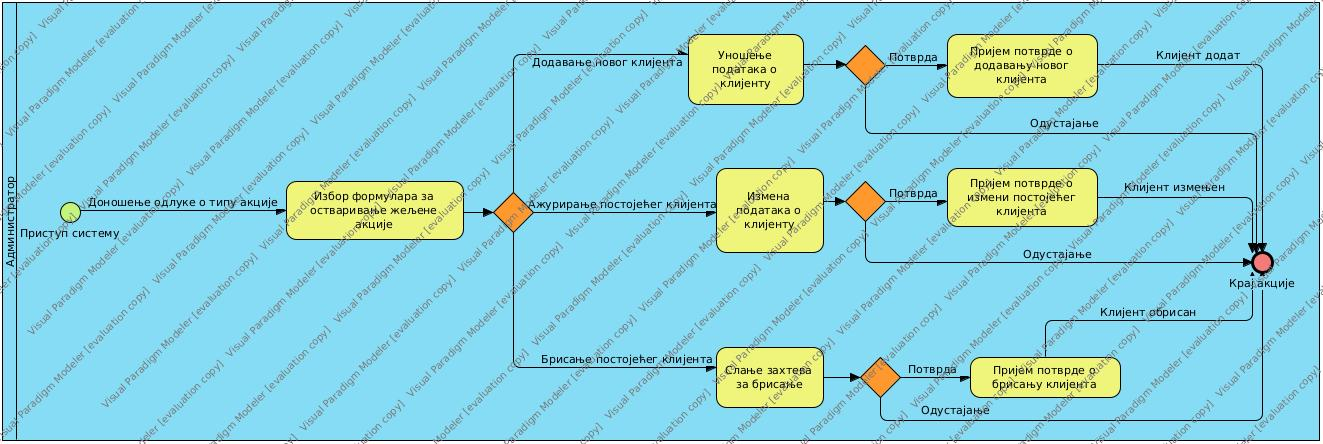
\includegraphics[angle = 90, scale = 0.35]{Slike/BPMNadministrativniPoslovi.jpg}
    \centering
    \caption{BPMN dijagram: Administrativni poslovi}
    \label{BPMN administrativni poslovi}
\end{figure}  